\documentclass[12pt]{article}
\usepackage[a4paper]{geometry}
\usepackage[myheadings]{fullpage}
\usepackage{fancyhdr}
\usepackage{lastpage}
\usepackage{graphicx, wrapfig, subcaption, setspace, booktabs}
\usepackage[T1]{fontenc}
\usepackage[font=small, labelfont=bf]{caption}
\usepackage{fourier}
\usepackage[protrusion=true, expansion=true]{microtype}
\usepackage[english]{babel}
\usepackage{sectsty}
\usepackage{url, lipsum}
\usepackage{enumerate}
\usepackage{enumitem}
\usepackage{mdframed}
\usepackage{soul}
\usepackage{xcolor}
\usepackage{amsmath}
\usepackage{amssymb}

\newcommand{\HRule}[1]{\rule{\linewidth}{#1}}
\onehalfspacing
\setcounter{tocdepth}{5}
\setcounter{secnumdepth}{5}
\pagenumbering{roman}

%-------------------------------------------------------------------------------
% HEADER & FOOTER
%-------------------------------------------------------------------------------
\pagestyle{fancy}
\fancyhf{}
\setlength\headheight{15pt}
\fancyhead[L]{Dylan-Matthew Garza and Elijah Sargeant}
\fancyhead[R]{Western Michigan University}
\fancyfoot[R]{\thepage}

%-------------------------------------------------------------------------------
% TITLE PAGE
%-------------------------------------------------------------------------------

\newcommand{\Prof}{Dr. Sawalha}
\newcommand{\Class}{ECE-5580: Computer Architecture}
\newcommand{\Assignment}{Final Project: Abstract}
\newcommand{\Specifics}{Superscalar Fixed-Length Vector Processor}
\newcommand{\Due}{Due: 4 November}

\begin{document}

\title{ \normalsize \textsc{}
		\\ [2.0cm]
		\HRule{0.5pt} \\
		\LARGE \textbf{\uppercase{\Assignment}}\\
		\Specifics\\
        \HRule{2pt} \\ [0.5cm]
		\normalsize \today \vspace*{5\baselineskip}}

\date{}

\author{
        Dylan-Matthew Garza \\
        Elijah Sargeant\\ 
        \Prof\\
        \Class\\
        \Due\\
        Western Michigan University \\
        Department of Electrical and Computer Engineering 
    }
\singlespacing
\maketitle
\break
\tableofcontents
\clearpage
\pagenumbering{arabic}
\section{Proposal}
\subsection{Project Objective}
The goal of this project is to comprehensively understand vector processors and
they achieve efficiency through handling data-parallel workloads. Vector processors
are a very important paradigm in regards to SIMD (Single Instruction Multiple Data) 
methodologies since they achieve parallelism by having parallel data operations. In this 
implementation, the the vector processor will be superscalar with out of order execution, in-order 
commit. In this implementation, the vector processor will support fixed-length vector sizes
of 32-bit.
\subsection{Methodology}
\subsubsection{Simulator Features}
A superscalar vector processor will require several components such as:
\begin{itemize}
    \item Multiple Functional Units for each lane on vector instructions
    \item Register Renaming Using RAT and RRAT 
    \item Vector Instruction Queue: Instruction queue to hold vector instructions
    \item Vector Pipeline Stages:

        \begin{itemize}
            \item Instruction Fetch
            \item Decode and Rename
            \item Dispatch
            \item Vector Execute
            \item Writeback/Memory Access
            \item Commit
        \end{itemize}
    \item Flexible Chaining of operation results to other
        Functional units and Load/Store Queue
    \item 4-Lane Vector Functional Units
    \item 4-Sets of Vector Funcional Units
\end{itemize}
\subsubsection{Input and Output}
\textbf{Input}
\begin{itemize}
    \item Trace file based on vector instructions 
    \item Number of execution lanes to functional units
\end{itemize}
\textbf{Output}
\begin{itemize}
    \item Number of vector instructions executed per cycle (IPC)
    \item Average IPC
    \item Maximum IPC
\end{itemize}
\subsection{Evaluation Plan}
The project will evaluate the efficiency of the implemented superscalar fixed-length pipeline. By
gathering information about the IPC, we can analyze how the number of lanes affect the IPC
of a fixed-length system. 
\section{Project Members}
\begin{itemize}
    \item Dylan-Matthew Garza:\\
        Responsible for writing the simulator and researching the related
        topics.
    \item Elijah Sargeant:\\
        Arbitrating the progress of the project as a whole and ensure correct
        implementation.
\end{itemize}
\break
\section{Block Diagram}
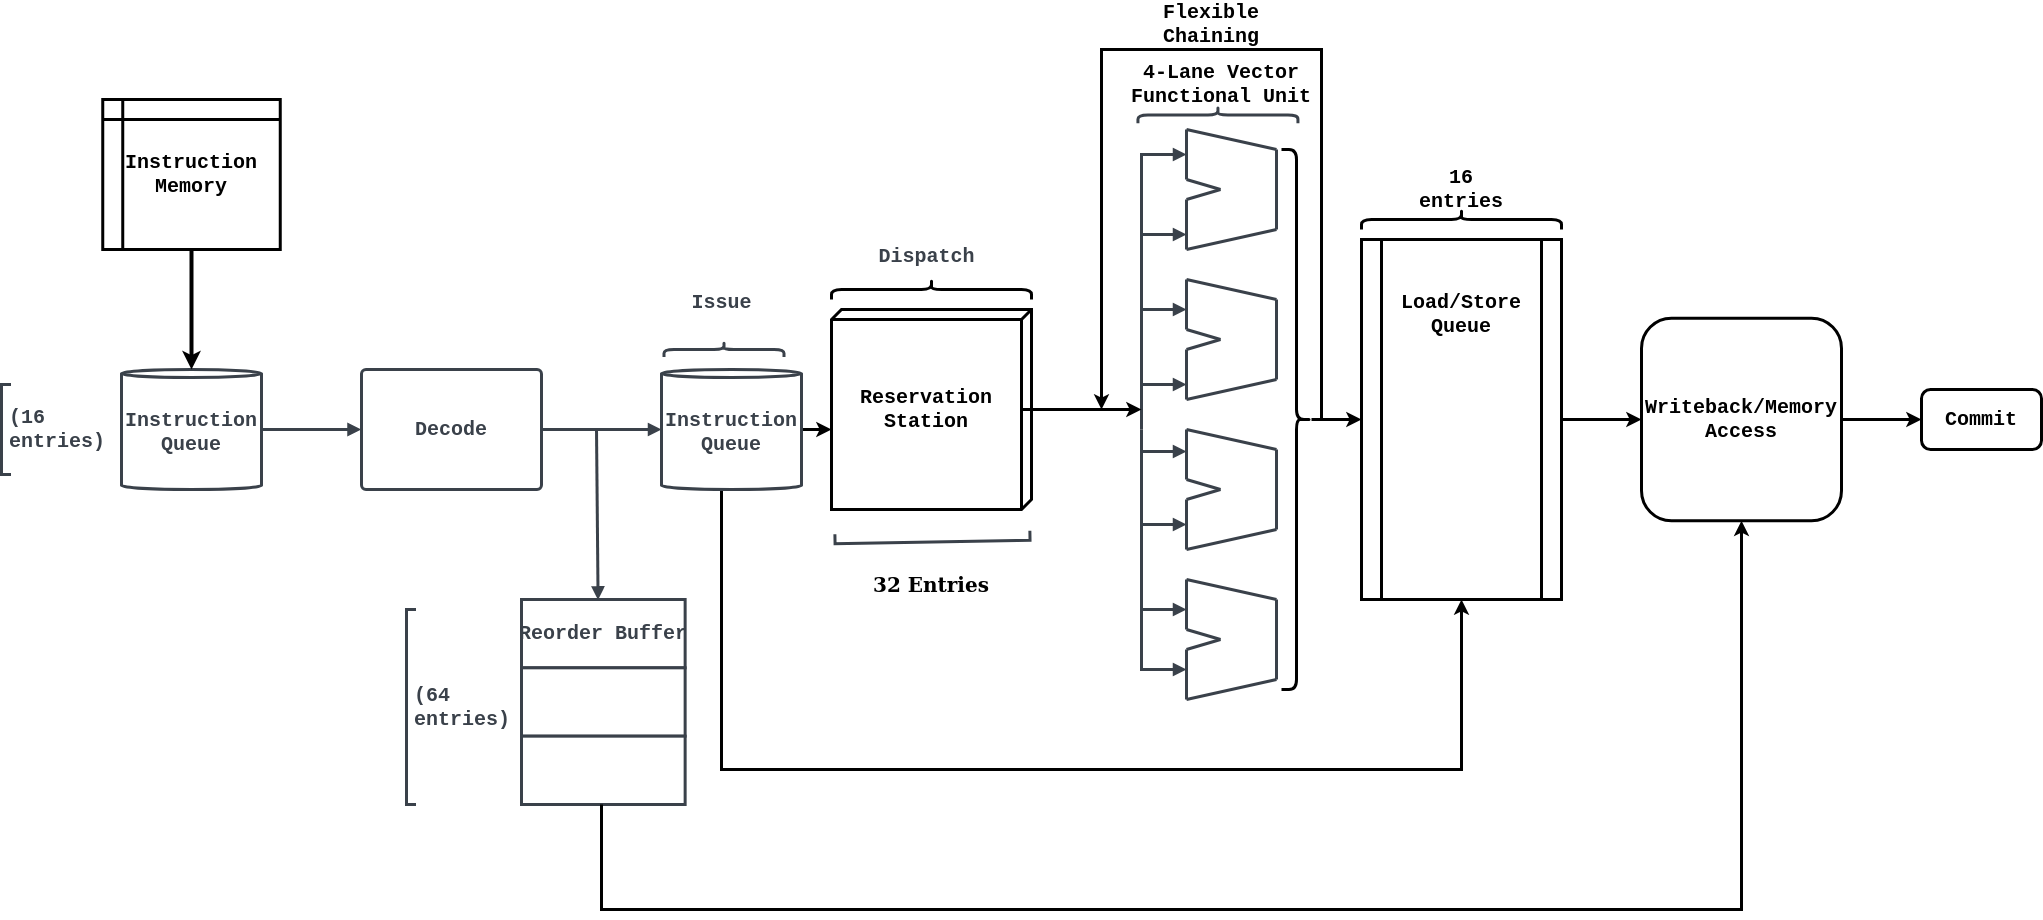
\includegraphics[scale=0.275]{diagram.png}
\captionof{figure}{Proposed Pipeline features to Simulate}
In this implementation, the exectution of vector instructions will not be limited
to the number of vector functional units, only by the number of lanes to each functional
unit.
\pagebreak
\section{References}

    \begin{verbatim}
    [1] R. Espasa, M. Valero and J. E. Smith, 
    "Out-of-order vector architectures," Proceedings of 30th Annual 
    International Symposium on Microarchitecture, Research Triangle 
    Park, NC, USA, 1997, pp. 160-170, doi: 10.1109/MICRO.1997.645807.
    \end{verbatim}
    \begin{verbatim}
    [2] K. Patsidis, C. Nicopoulos, G. C. Sirakoulis and G. Dimitrakopoulos, 
    "RISC-V2: A Scalable RISC-V Vector Processor," 2020 IEEE 
    International Symposium on Circuits and Systems (ISCAS), Seville, 
    Spain, 2020, pp. 1-5, doi: 10.1109/ISCAS45731.2020.9181071.
    \end{verbatim}
    \begin{verbatim}
    [3] S. S. Chen and A. J. Schiffleger, “Flexible chaining in 
    vector processor with selective use of vector registers as 
    operand and result registers ,” Apr. 28, 1987
    \end{verbatim}
    \begin{verbatim}
    [4] Di Mascio, Stefano & Menicucci, Alessandra & Gill, Eberhard 
    & Monteleone, Claudio. (2023). Extending the NOEL-V Platform with 
    a RISC-V Vector Processor for Space Applications. Journal of Aerospace 
    Information Systems. 20. 1-10. 10.2514/1.I011097. 
    \end{verbatim}

\end{document}
